\documentclass[10pt]{article}
\usepackage{float}
\RequirePackage{eso-pic}
\usepackage{caption}
\captionsetup[table]{labelformat=empty}



\usepackage{geometry}
\geometry{
a4paper,
left=11mm,
right=14mm,
top=37mm,
bottom=14mm,
}



\usepackage{colortbl}
\usepackage{fontspec}
\setmainfont[Ligatures=TeX]{Calibri}



\newcommand\BackgroundPic{%
\put(0,0){%
\parbox[b][\paperheight]{\paperwidth}{%
\vfill
\centering
\includegraphics{MBIE_generic_background.pdf}%
\vfill
}}}



\begin{document}
\thispagestyle{empty}
\AddToShipoutPicture{\BackgroundPic}
\section*{Key Export Statistics\footnotemark - Berries\footnotemark }
Published on April 11, 2016. \par
\small{\noindent{\textit{Monthly data from January 2000 to November 2015.}}}
\begin{table}[ht]
\centering
{\scriptsize
\begin{tabular}[t]{p{1.8cm}>{\hfill}p{1.4cm}>{\hfill}p{1.4cm}>{\hfill}p{1.6cm}>{\hfill}p{1.9cm}>{\hfill}p{2cm}>{\hfill}p{1.9cm}>{\hfill}p{1.5cm}}
 \textbf{Country} & \textbf{Yearly Qty} & \textbf{Yearly Value} & \textbf{Yearly Price} & \textbf{3Year CAGR(Qty)} & \textbf{3Year CAGR(Value)} & \textbf{3Year CAGR(Price)} & \textbf{Price Elasticity} \\
\hline
Australia & 1,137 & 22.0 & \$19.3 & 3.6\% & 8.2\% & 4.4\% & 0.8 \\  
China & 1,291 & 4.5 & \$3.5 & 24.8\% & 43.5\% & 15\% & 1.7 \\  
USA & 248 & 2.6 & \$10.4 & 23.4\% & 24.6\% & 0.9\% & 25.3 \\  
Japan & 383 & 1.5 & \$3.8 & 23.6\% & 22.9\% & -0.5\% & -44.5 \\  
Thailand & 41 & 0.7 & \$16.1 & 6\% & 39.9\% & 32\% & 0.2 \\  
Taiwan & 39 & 0.6 & \$15.7 & 27.8\% & 54.2\% & 20.7\% & 1.3 \\  
Other & 164 & 2.2 & \$13.3 & 47.3\% & 34.7\% & -8.5\% & -5.5 \\  
Total & 3,302 & 33.9 & \$10.3 & 15.8\% & 15.1\% & -0.7\% & -23.9 \\  
\hline
\end{tabular}
}
\caption{\scriptsize Top 6 Berries Markets for year ending November - 2015: Quantity('000 kg) Value(NZ\$Mill), Price and their last 3-Year Growth Rates}
\end{table}


\vspace{-0.7cm}



   \begin{figure}[H]
   \centering
    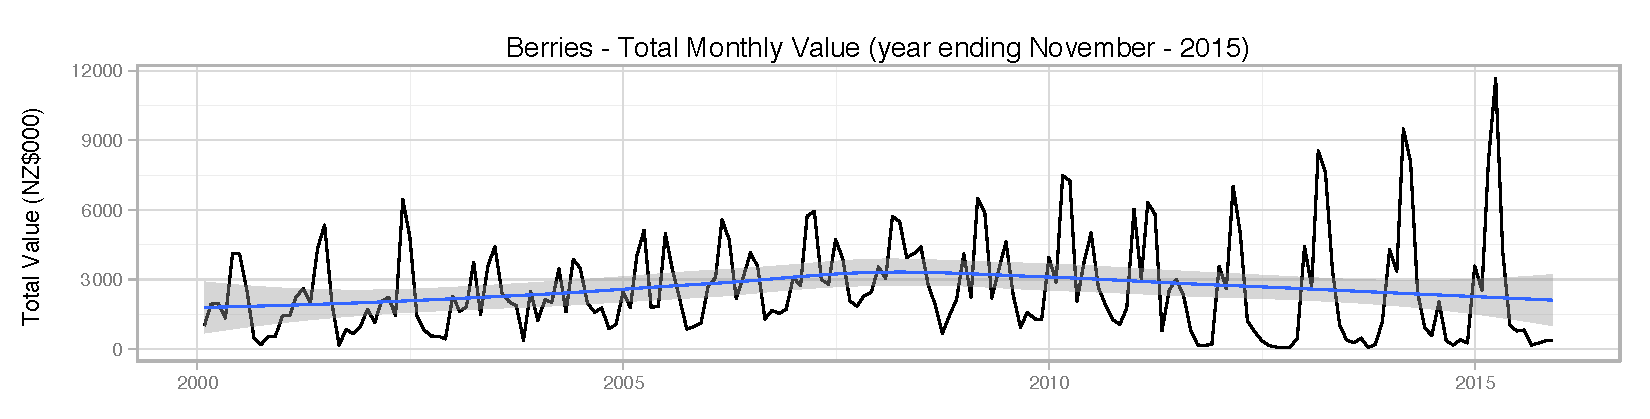
\includegraphics[scale=0.53]{../graphs/monthly_value/berries_monthly_value.pdf} \
    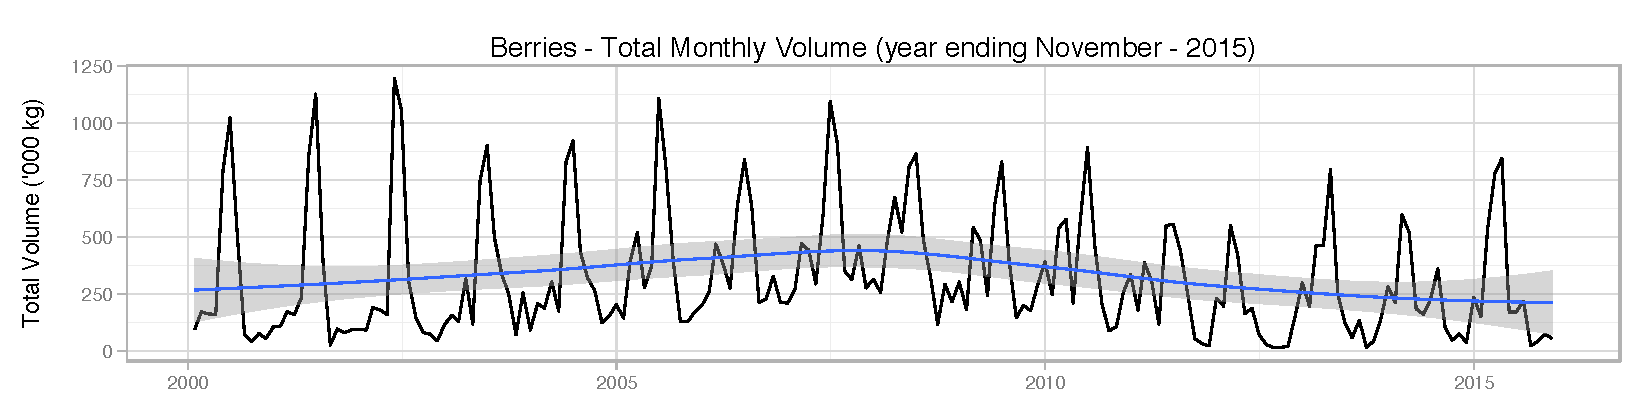
\includegraphics[scale=0.53]{../graphs/monthly_volume/berries_monthly_volume.pdf} \
    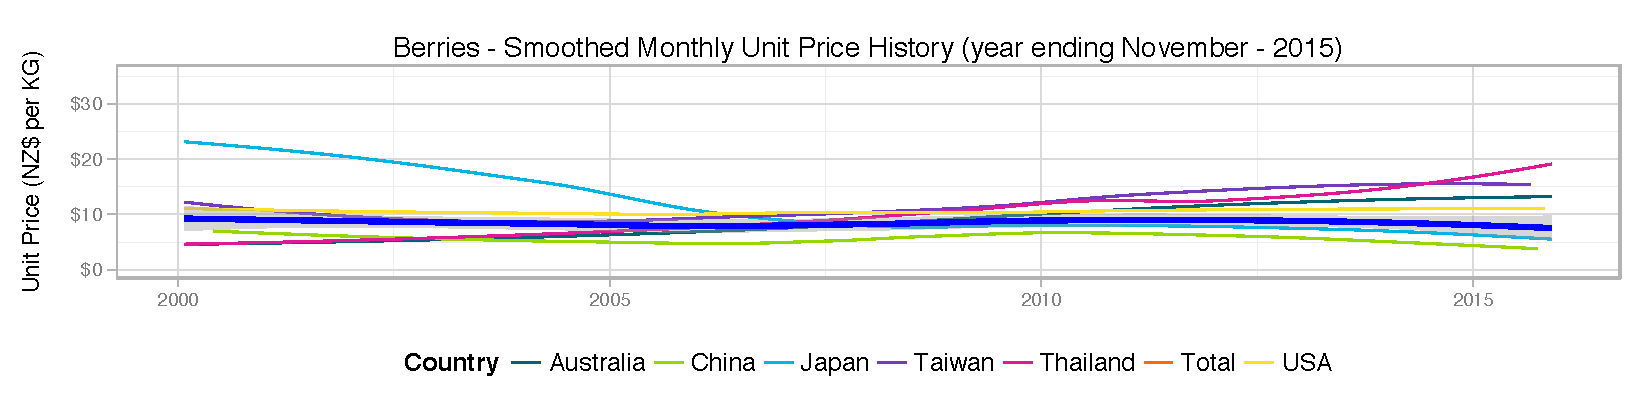
\includegraphics[scale=0.53]{../graphs/smoothed_price/berries_smoothed_price.pdf} \
    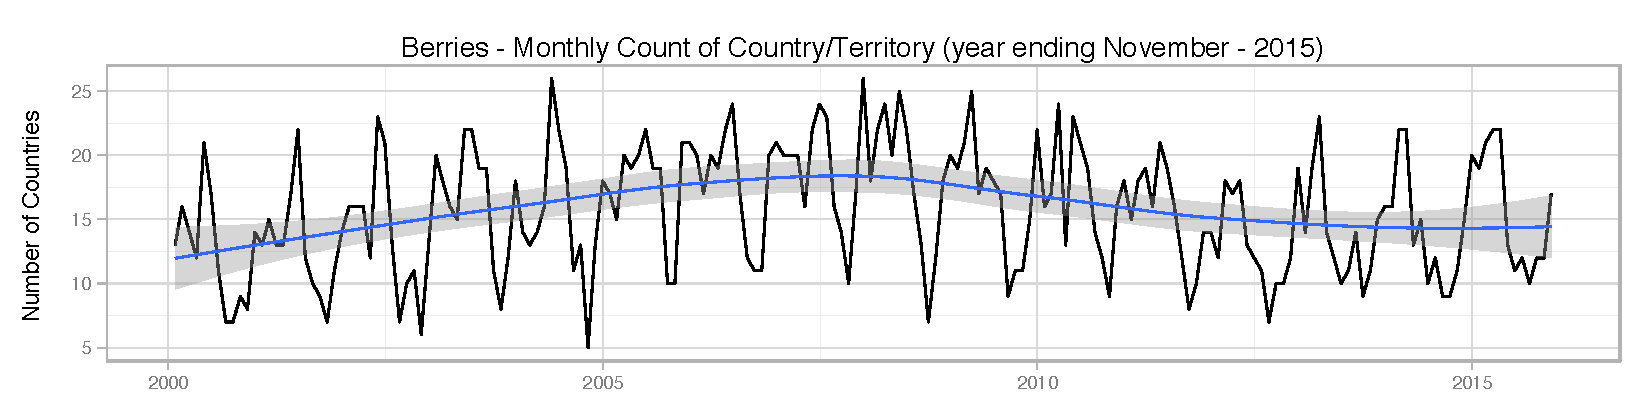
\includegraphics[scale=0.53]{../graphs/monthly_number_countries/berries_monthly_count.pdf} \
    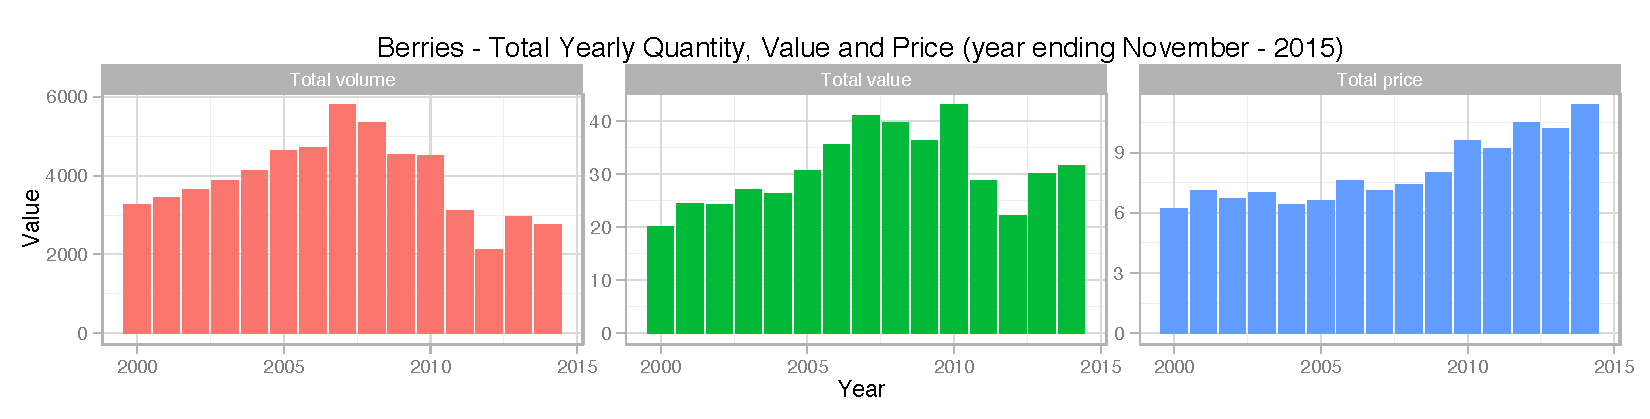
\includegraphics[scale=0.53]{../graphs/yearly_summary/berries_yearly_summary.pdf} \
   \end{figure}



\footnotetext[1]{Source: Statistics New Zealand - Overseas Merchandise Trade}
\footnotetext[2]{Harmonised System Codes for Berries starting with: 081040, 081090, 081120.}
\end{document}
